\chapter{\ac{KIEMConfig} Plug-in}
\label{chapter:KiemConfig}
This chapter describes the contents and functionality of the newly created
plug-in to solve the problems described in Chapter \ref{chapter:ConfTask}.
A new plug-in was created in order to improve modularity within the \ac{KIELER} framework.
Putting the code into the \ac{KIEM} plug-in itself would have meant that
there would have been no way to separate the two projects.

The sections in this chapter describe the different parts of the \ac{KIEMConfig} plug-in.
The whole plug-in is structured according to the Model-View-Controller pattern.
The first section will describe the data storing classes which constitute the model.
The second section will describe the different manager classes which are essentially the
controller of the entire plug-in. This section will also look at the \ac{API} that the
\ac{KIEMConfig} plug-in provides to other plug-ins.
The last section will describe the classes that render the preference pages and other
view elements.

\section{Data Classes and Utilities - the Model}
\label{section:ConfModel}
This section will describe the different classes that are responsible for storing all
data that the plug-in needs at runtime.


\subsection{ConfigDataComponent}
\label{section:ConfigDataComponent}
\index{ConfigDataComponent}
This extension to the AbstractDataComponent of the \ac{KIEM} is responsible for solving
the problem described in Section \ref{section:ConfTaskConfig} and implements the behavior
described in Section \ref{section:ConfConceptsConf}. The component is a DataComponent
like all others used in the \ac{KIEM}. It is registered through the extension point
that allows new DataComponents to appear in the list of available components.
However unlike the usual DataComponent that is responsible for simulating a model during
an execution run its main function is to store the configuration of the \ac{KIEM}.

Like all other DataComponents the ConfigDataComponent contains an array of
KIEMProperties. These properties contain a String key which should be non-null and unique and 
a value which can be of various types. However for the purpose of storing configuration
elements only the String value will be used.

The new DataComponent also provides additional methods in order to make accessing and manipulating the
array more convenient:
\begin{description}
 \item \textbf{KiemProperty findProperty(String key)} : This method iterates through the array and attempts
to find the KiemProperty that has exactly the provided key. Since the keys are assumed to be unique the first
match is returned by this method. If there is no property with the given key the method will throw
an Exception.
 \item \textbf{void removeProperty(String key)} : This method attempts to remove the property identified by
the given key from the array. It does this by converting the array to a list, locating and removing the
specified property and then converting the list back to an array. This procedure may not be as efficient
as manually constructing the new array but it still performs the operation in linear time. Furthermore
it makes the method easier to understand than the alternative.
 \item \textbf{KiemProperty updateProperty(String key, String value)} : This method updates the property 
identified by the key with a new value. It first checks if the property already exists and if it does its value
is updated. If a property with the specified key doesn't exist a new one is created and the provided value
stored inside.
\end{description}

In addition to those methods the ConfigDataComponent also keeps a reference to its DataComponentWrapper (see Section
\ref{section:IntroDataComponentWrapper}). This is necessary in order to retrieve the properties from the wrapper
right after the execution file was loaded and to write them back into the wrapper before the file is saved.

The ConfigDataComponent is not only used to store the properties of the currently active configuration that each
execution file carries. However it is also used to store the default configuration that is saved in the Eclipse
preference store. This is done because both instances are closely linked and have the same requirements
(see Section \ref{section:CurrentConfiguration}).

The default behavior of the Configuration Manager is to add a new ConfigDataComponent to each execution file
that it encounters. However as this feature can be turned off the user also has can upgrade old files or
downgrade new ones by manually adding and removing the ConfigDataComponent.


\subsection{EditorDefinition}
\label{section:EditorDefinition}
\index{EditorDefinition}
The EditorDefinition class is responsible for storing information about the editors that are known to
the \ac{KIEMConfig}. Each instance of this class stores the information about a single editor. This is
necessary in order to successfully operate a list of execution files that work for the currently active
editor.
\begin{description}
 \item \textbf{String editorId} : The identifier for the given editor. This attribute is a unique non-null String
by which any editor can be identified. For example the standard Java editor has the id \textit{org.eclipse.jdt.ui.CompilationUnitEditor}.
 \item \textbf{String name} : The name of the editor. This is the human readable name given to the editor
by the plug-in that defines the editor. Storing this attribute may seem redundant since the names of
the editors can be retrieved through an Eclipse mechanism if the editor id is known. However there is no
guarantee that a previously saved editor id exists in the currently active application in which case the name
of the editor can't be retrieved.
 \item \textbf{boolean isLocked} : This attribute is responsible for showing that the editor can not be removed.
The reason that an editor might become read only will be explained in Section \ref{section:DefaultSchedule}.
\end{description}

\subsection{ScheduleData}
\label{section:ScheduleData}
\index{ScheduleData}
The ScheduleData class is responsible for tracking the different execution files that are known
to the \ac{KIEMConfig}. A ScheduleData object is the representation of a single execution file. 
These objects are used to main he lists of recently used schedules and of those that match the 
currently opened editor. It contains the following attributes:
\begin{itemize}
 \item The most important attribute is the path at which the execution file that this instance
should represent is located. The path is used to trigger the loading of the file inside
the Execution Manager. It is also used to determine whether a newly loaded execution file
is already known. The path also doubles as the unique identifier for the schedule since there
can't be two files at the same physical location.
\item The ScheduleData object also stores a list of priorities for all known editors. This is
necessary in order to determine whether or not a given schedule can be used with the currently
opened editor and which position it should have in an ordered list. To make accessing and manipulating
this list easier it simply uses an instance of the ConfigDataComponent. The component already has
methods for accessing the array inside and can be easily stored and loaded.
 \item Like the EditorDescription a ScheduleData also contains a boolean \textbf{isLocked}. ScheduleData
object with that attribute set to \textit{true} can't be modified or removed (see Section \ref{section:DefaultSchedule}).
\end{itemize}

\subsection{Tools}
\label{section:Tools}
The Tools class holds a host of useful methods and attributes that are used in various parts of the plug-in.

\subsubsection{Attributes}
\label{section:ToolsAttributes}
First of all it contains messages and tool tips that are used in more than one class.
This ensures that the appearance of the different messages is unified across the entire plug-in. It also
makes it easy to change these messages or combine different partial messages to new ones.

The class also holds the different identifiers for the properties that are used in the plug-in. This is done
to avoid bugs due to mistyping an identifier which is likely to happen if it is stored in two different places.

\subsubsection{Methods for Parsing and Serialization}
\label{section:ToolsMethodsParsing}
All of the manager classes in the \ac{KIEMConfig} need to save their properties into the Eclipse preference store.
In order to have the information stored in a structured way an \ac{XML} like format was chosen. As this requires the keys and values
to be formatted in a certain way the Tools class provides methods to format the Strings in the required way.
\lstset{
backgroundcolor=,
}
\begin{description}
 \item \textbf{String putValue(String key, String value} : Converts the (key, value) pair into a formatted String for saving
into the Eclipse preference store. The resulting String has the following format: 
\lstinline|<[key]>[value]</[key]>|.
 \item \textbf{String putProperty(KiemProperty property} : Convenience method for transforming a KiemProperty object into a
formatted String. This method exists because most of the items serialized in this way are of that type. The resulting String
has the following format: \lstinline|<KIEM_PROPERTY><Key>[property.key]</Key><Value>[property.value]</Value></KIEM_PROPERTY>|.
\end{description}

The methods described above provide all the necessary facilities for the \ac{KIEMConfig} to save its preferences
into the Eclipse preference store. In order to retrieve these properties the Tools class provides another set of
methods. These methods take an input String and try to parse the saved properties.
\begin{description}
 \item \textbf{String getValue(String key, String input)} : This method retrieves the value enclosed by tags with
the given key. The retrieved value can either be an atomic String that can directly be assigned to a property or
another series of values enclosed in their tags. The method will always look for the outermost tags inside the
input String. The method returns null if there are no tags with the provided key inside the input String.
 \item \textbf{KiemProperty getKiemProperty(String input)} : This convenience method tries to retrieve the 
(key, value) pair that constitutes a KiemProperty object from an input String.
 \item \textbf{String[] getValueList(String key, String input)} : Since there sometimes is the need to store an entire
list of entities the Tools class provides a method to convert an entire list back to the individual Strings.
The method iterates over the input String and extracts all elements that are enclosed in tags with the specified key.
\end{description}


\subsubsection{Methods for Dialogs}
\label{section:ToolsMethodsDialogs}
The Tools class also contains methods for easily displaying error and warning dialogs.
These methods take the information, add the own plug-in id and forward the information to the 
error handling facilities inside the Execution Manager itself.


\subsection{MostRecentCollection}
\label{section:MostRecentCollection}
The MostRecentCollection is a new collection type that is can be used for simulating the 
behavior found in 'Open recent' menu item of almost any text editing application.
To avoid the list growing too long it can be given a maximum capacity. After that capacity
is reached the oldest entry will be deleted when a new one enters the list.
The default implementation of the collection uses an ArrayList to store the data but any
other list works as well. Most operations are directly delegating to the operations of the 
underlying List. 
The only exception is the add(item : T) method that works in a different way:
\begin{enumerate}
 \item It checks if the item is already in the list and removes it. This is done to ensure
that already added items don't appear twice in the list.
 \item It adds the item at the highest index to the end of the list and increments the index of all other items.
 \item The element at the head of the list is overridden by the new item.
 \item Optionally the last item is removed if the list has grown beyond the capacity.
\end{enumerate}
The collection also provides an additional method that is used to replace an item in
the list by another one. This is used when files are renamed and the name of the ScheduleData inside
the list has to be updated.

This collection is used to track the most recently used schedules and display them
in the corresponding ComboBox.



\section{Manager Class - the Controller}
\label{section:ConfController}
The manager classes are responsible for the control flow inside the plug-in. They gather information
from the view, the Eclipse preference store and the Execution Manager and create and update a
model using the classes described in Section \ref{section:ConfModel}. There are multiple managers
each with a different task:
\begin{itemize}
 \item The \textbf{Configuration Manager} is responsible for maintaining the configuration saved in
each execution file and the default configuration saved in the preferences store.
 \item The \textbf{Schedule Manager} is responsible for keeping track of the different
execution files and updating the information inside the ScheduleData objects.
 \item The task of the \textbf{Editor Manager} is to
\end{itemize}



\subsection{Abstract Manager}
\label{section:AbstractManager}
All of the managers share some common features that each of them must provide. Some of those
features are handled almost the same or exactly the same in each manager. This lead to the creation
of an abstract super class for all managers (see Figure  %\ref{fig:AbstractManagerUML}) 
that takes care of the basic tasks.

The first task is to allow other classes to register as a listener to the manager. Some of the classes
in the \ac{KIEMConfig} have to perform updates when a value inside the model changes. It is the managers
responsibility to inform the listeners when such a change was completed successfully.

The second task is to provide the subclasses with facilities to easily access the Eclipse Preference Store.
Whenever a value is requested by any part of the controller or another plug-in and a manager didn't access
the preference store yet it has to gain access to the store and retrieve the information belonging to it.
Furthermore when the user explicitly wants to save the preferences or the workbench is shutting down the
data contained in the model has to be saved into the Eclipse Preference Store. For an example of a 
saved configuration see Appendix \ref{section:AppendixSavedConf}).


\subsection{Configuration Manager}
\label{section:ConfigurationManager}
\index{Configuration Manager}
The Configuration Manager basically handles all the problems described in Section \ref{section:ConfTaskConfig}.
This means that the Configuration Manager has two responsibilities:
\begin{enumerate}
 \item It manages the configuration contained in the currently opened execution file and all properties contained in
it. It is also responsible for deciding whether or not the preferences stored in that configuration should be used
or the default preferences instead.
 \item It manages the default configuration that the user can access and modify through the preference pages 
(see Section \ref{section:ConfView}). For all of the predefined properties it also has to hold and manage the 
hard-coded default values.
\end{enumerate}

\subsubsection{Currently Loaded Configuration}
\label{section:CurrentConfiguration}
\index{Current Configuration}
The first thing the Configuration Manager has to do when a request for the value of a property is made
is to locate the ConfigDataComponent that contains the property. 

It first takes a look at the list of keys where the default configuration should be used. If this is the case the task is quite simple
and the default configuration is loaded from the preference store and used. If the current configuration
should be used the task is a little more difficult. The Configuration Manager then has to look at the
DataComponentWrapperList inside the Execution Manager where all components for the currently opened
execution file are stored. If the list already contains a wrapper with the ConfigDataComponent inside
that component is used. Otherwise a new ConfigDataComponent is created, initialized with the default values
from the default configuration and then added to the list of the current execution file. Since this feature
can be disabled by the user the Configuration Manager can encounter execution files that have no ConfigDataComponent
or where the component simply doesn't contain the requested value. In this case the default configuration has
to be used.

If the default configuration couldn't supply a value the last possibility is that the caller passed a non-null default 
value for the given property. In this case the default value is returned to the caller. 

If no value could be retrieved in the way described above there is no way to get a valid value for the requested key. 
In this case the Configuration Manager notifies the caller through an exception of these circumstances.

However if the value was expected in the current configuration but not found the Configuration Manager assumes 
that it should have been in there. To remedy that situation the Configuration Manager will try to add a new property 
to the current configuration with the value that the method will return (either the one retrieved from the default 
configuration or the default supplied by the caller).


\subsubsection{Default Configuration}
\label{section:DefaultConfiguration}
\index{Default Configuration}

The first responsibility of the Configuration Manager with respects to the default configuration is to manage
the hard-coded default values. The whole idea of the \ac{KIEMConfig} is to avoid using hard-coded values
and retrieve user defined values. However the Execution Manager and the \ac{KIEMConfig} rely on certain values
to be present and even though the user is encouraged to change them they still have to be present before the user
enters them for the first time. Furthermore the user may want to revert back to sensible default values which
should be provided by the plug-in itself.

This means that the plug-in contains a list of hard-coded default values for the needed properties.
It also supplies methods to access these properties and restore the default values by writing their values
into the default configuration.

\lstset{
backgroundcolor=,
}
The next feature that the default configuration supplies has to do with adding new ConfigDataComponents to the
list inside the Execution Manager. Since the Configuration Manager knows which properties will be taken from
the current configuration it can already make sure that the component contains some value. This is done
through calling \lstinline|void initWithDefaults(AbstractDataComponent dataComponent)| with the newly created component.
This causes the default values for all properties that are likely to be taken from the current configuration to
be added to it.

The Configuration Manager also supplies different views on the default configuration. 
\begin{enumerate}
 \item \textbf{KiemProperty[] getDefaultConfig().getProperties()} : This method simply returns all properties
stored in the default configuration. This is the list actually written to the Eclipse preference store.
 \item \textbf{KiemProperty[] getInternalDefaultProperties()} : This method returns the list of properties that
are needed to operate the Execution Manager and the \ac{KIEMConfig}. The motivation for this method is that
the keys and types for these values are already known. That means that a view that modifies these properties
can be designed in a more user-friendly way than would have been possible otherwise. Furthermore the Configuration 
Manager is guaranteed to have hard-coded default values for these properties.
 \item \textbf{KiemProperty[] getExternalDefaultProperties()} : This method returns the complement of the internal
properties with respect to the entirety of the default properties. These properties are those that the user defined
himself.
\end{enumerate}
However neither of the last two lists will return the default editor as that falls into the responsibility of
the Editor Manager which is described below.

The Configuration Manager also supplies methods to add new properties to the default configuration, remove properties
and update the value of specific property.

\subsection{Schedule Manager}
\label{section:ScheduleManager}
\index{Schedule Manager}
The Schedule Manager is the second of the two large managers. It is responsible for managing the
ScheduleData object, the execution files and provide the methods for solving the problem described
in Section \ref{section:ConfTaskEasyLoading}. These responsibilities can be broken down into
six different parts:
\begin{enumerate}
 \item Gather the different types of lists of schedules.
 \item Manage the different ScheduleData objects and provide methods to add, remove and change
them.
 \item Deal with loads and saves triggered through the normal workspace interface.
 \item Provide a means to trigger the loading of an execution file in the Execution Manager.
 \item Track the locations of the execution files if the user modifies them.
 \item Loading the default schedules.
\end{enumerate}


\subsubsection{Provide the Schedule Lists}
\label{section:ProvideScheduleLists}
The Schedule Manager stores all ScheduleData objects in one list that is saved and loaded through
the abstract super class. However different components of the \ac{KIEMConfig} or other plug-ins 
need different views on that list. Some components may not want to display all schedules or have
the list sorted in a certain way. To provide these different views the Schedule Manager contains
several methods:
\begin{description}
 \item \textbf{List<ScheduleData> getAllSchedules()} : Returns the list of all schedules. This
method triggers a load through the super class if no load has been performed yet. It also triggers
a load of the default schedules described at the end of Section \ref{section:DefaultSchedule}.
 \item \textbf{List<ScheduleData> getMatchingSchedules(String editorID, String editorName)} :
This method is responsible for constructing the list that will be displayed in the ComboBox that
shows the list of schedules matching the currently active editor. First it tries to find an
EditorDefinition with the given editor id. If that fails a new EditorDefinition is created and
added it to the list of known editors. After that the method searches through the list of
all schedules and extracts those that have a positive priority for the given editor. The list
is then sorted  and returned with the editor with the highest priority appearing at the lowest index.
 \item \textbf{List<ScheduleData> getRecentSchedules()} : This method constructs the list of 
recently used schedules. This list is used in another ComboBox to allow the user to easily load
his last used schedules. In order to realize this feature the Schedule Manager keeps a list of
all execution file locations that were recently accessed using the list described in Section
\ref{section:MostRecentCollection}. When the method is called it iterates over the list of locations
and tries to find a schedule for each location. Schedules that match a location in that list are 
added to the resulting list. Entries in the list of locations where no schedule can be found will
be removed from the list as they are no longer valid.
 \item \textbf{List<ScheduleData> getImportedSchedules()} : Returns the list of default schedules.
This feature will be described in detail at the end of Section \ref{section:DefaultSchedule}.
\end{description}


\subsubsection{Listen to User Events}
\label{section:UserEvents}
It has to be assumed that the user creates his own schedules and saves and loads them through the workspace explorer.
Since the Schedule Manager should attempt to track all available execution files it has to be informed about
these changes and act on the notification. In order to get notified the Event Listener extension point
of the Execution Manager is used (see Section \ref{section:EventListener}). The listener will dispatch and event
that contains the location of any saved or loaded execution file as soon as the user performs the corresponding action.
When the Schedule Manager receives such an event it will perform the following steps:
\begin{enumerate}
 \item Try to find a schedule with the provided location. If a schedule can be found there is nothing to be
done and the method skips to the last step.
 \item If no schedule was found with the given location a new one has to created. In order for that the method
first has to check if there is an active editor and if the editor is known to the Schedule Manager. If that is
the case the method skips ahead to step 4.
 \item If the editor is unknown it is created. If no editor is active the default editor will be used.
 \item The new schedule is created with the editor determined in the previous steps. Since it is assumed that
the created schedule works with the currently active editor a default priority is inside to that editor in the
newly created schedule.
 \item Since the file operation constitutes a use of the given schedule the list of recently used schedules has
to be updated. The used schedule will be added to the top or moved to the top if it's already inside.
\end{enumerate}


\subsubsection{Open a Schedule}
\label{section:OpenSchedule}
The Schedule Manager also provides a way to trigger a load in the Execution Manager. This is
done through the modified method described in Section \ref{section:ConfKiemOpenFile}. The reason for this
is that the Schedule Manager may try to load schedules where the files no longer exist or that the 
Execution Manager is unable to load. The method mentioned above will throw Exceptions in order to perform
the caller of these circumstances and the Schedule Manager will inform its callers.

As described in the last section the Schedule Manager will be informed of a load through the Event Listener
interface and will act on it. However if the load is triggered by the Schedule Manager itself that behavior
would not be desirable. To avoid the Schedule Manager informing itself the method makes sure that the next
event indicating a loaded file will be ignored.

Since the load triggered by the Schedule Manager constitutes an access to that file the associated schedule
is added to the list of recently used schedules. Furthermore all listeners on the Schedule Manager will
be notified since view updates may be necessary.


\subsubsection{Tracking Execution Files}
\label{section:TrackingExecutionFiles}
As described above new schedules will be created when the user manually loads or saved an execution file.
However in some cases the user may also choose to remove, rename or move execution files. Since the Schedule Manager
relies on the path of the execution file to load the schedules it runs into trouble if the path is changed outside
its control.

The only solution in this case is to prompt the user to select a new path for an execution file that is no
longer at the expected location. An alternative would be to simply delete the schedule and all assigned priorities.

\lstset{
backgroundcolor=,
}

However if the user performs a remove, rename or move through the context menu inside the Eclipse workspace window
Eclipse itself provides a way to get notified of these changes. Any class can register themselves as listener
by calling : 
\lstinline|RefactoringCore.getHistoryService().addHistoryListener(IRefactoringHistoryListener listener)|.
Whenever the removal, renaming or moving of a file completes all listeners will be notified through a call to
\lstinline|void historyNotification(RefactoringHistoryEvent event)|. The event contains different information
based on the type of the operation. Depending on the type of operation that was performed the Schedule Manager
takes one of the following actions:
\begin{description}
 \item \textbf{Delete} : One or more files were deleted by the user. In this case the event contains the list
of files that was deleted. Since the user has no more use for the deleted files he probably has no use for
the schedule and the saved priorities as well. The Schedule Manager attempts to find the ScheduleData object
associated with the given file and removes it.
 \item \textbf{Rename} : The user changed the name of a file. The event provides the old file name and the 
new name of the file. In order to keep track of the file the Schedule Manager tries to find the ScheduleData
associated with the old file name and changes the name to the new file.
 \item \textbf{Move} : One or more files were moved by the user to a new location. The event contains the list
of files that were moved and the destination path. The Schedule Manager tries to find a Schedule for each
of the files involved and changes its name to reflect the new location.
\end{description}


\subsubsection{Default Schedule}
\label{section:DefaultSchedule}
\index{Default Schedule}
\index{Extension point}
An additional requirement that came up through the development of this project was that it would
be desirable to provide the user with an initial set of execution files that are not located inside
the users workspace.

For that purpose the new extension point seen in Listing \ref{list:DefaultSchedule} was created.
\listingxml
\showlistingex{code/defaultSchedule.txt}
{XML}
{Example implementation of the Default Schedule extension point.}
{list:DefaultSchedule}
{t}

As soon as the Schedule Manager loads the schedules from the Eclipse preference store it also triggers
a load from the components registered on this extension point. The new schedule will be constructed with
the location provided through the corresponding field in the extension point. After that the Schedule Manager
iterates through the list of child elements of a given execution file and adds all the editors and their
priorities to the schedule and the Editor Manager.

Since the schedules and editors added in this way are supposed to be a kind of factory defaults they are not
supposed to be removed or changed. The Schedule Manager sets a field in both the newly created ScheduleData
objects and the EditorDefinitions. It is the responsibility of the different view elements not to modify
entities marked in this way.


\subsection{Editor Manager}
\label{section:EditorManager}
\index{Editor Manager}
As described in Section \ref{section:EditorDefinition} the editor names and editor ids have to be saved
since they might not be available in the current runtime environment. The Editor Manager is responsible
for managing the list of all known editors. It also contains facilities around the default editor.

\begin{description}
 \item \textbf{EditorDefinition addEditor(EditorDefinition editor} : Adds a new editor to list of 
editors and return the added editor. If an editor with that editor id already exists in the list it is
not added to prevent duplicates. In this case the already existing editor is returned instead. Since
some methods may want to work on the editor that was just added they can work on the returned reference
instead of having to perform a find to get the correct object.
 \item \textbf{EditorDefinition findEditorById(String id)} : This method searches through the list
of available editors to retrieve the editor with the given id. Since editors ids are assumed to be
unique the first match is returned. This method is for example used to build the list of schedules that
work with the currently active editor.
 \item \textbf{void removeEditor(EditorDefinition editor)} : At some point the user may decide that
one of the editors is no longer used. In this case the editor is simply removed from the list of
available editors. However if the removed editor is the default editor (see Section \ref{section:DefaultEditor})
the method also has to choose a new default editor. The editor of choice for simplicity is the first
editor in the list. If the last editor is removed a hard-coded default editor is restored.
\end{description}

When the user is finished changing the editors the manager can use the facilities in the super class to
write the list of known editors to the Eclipse preference store.


\subsubsection{Default Editor}
\label{section:DefaultEditor}
\index{Default Editor}
The \ac{KIEMConfig} contains a facility for showing the list of schedules that match the currently active
editor. However there may be situations no editor is opened. Since the user should be able to keep working
with his schedules in this situation there is the need to define a default editor. This editor will be assumed open 
when in fact no editor is active.

Although the actual storing of the default editor happens inside the Configuration Manager the Editor Manager
still supplies facilities to get and set the default editor. This arrangement is more intuitive than having
the methods inside the Configuration Manager.


\subsection{Contribution Manager}
\label{section:ContributionManager}
\index{Contribution Manager}
The Contribution Manager is responsible for maintaining the view elements (see Section \ref{section:ScheduleSelector}) 
that are not part of any of the preference pages. To accomplish this the manager has two tasks:
\begin{enumerate}
 \item The manager must create the view elements and store them. As described in Section 
\ref{section:ToolbarContributionProvider} the Execution Manager will ask the \ac{KIEMConfig}
for the list of items it wants to contribute to the tool bar. The manager then has to 
create the list with the saved view elements and forward it through the extension point.
 \item As the user might want to hide the new elements the Contribution Manager also has to 
keep track of the visibility of the elements. Showing and hiding the components is realized
in the following way:
\begin{itemize}
 \item When the Execution Manager requests the list of control contributions the Contribution Manager
checks whether or not the given view element should be visible. If it should not be shown on the tool bar
it is not added to the list and thus never reaches the tool bar.
 \item When the user changes the visibility of a given view element the manager first updates its own
representation of that information and triggers a save into the Eclipse preference store through the use
of the facilities in the super class. After that the manager triggers a refresh in the Execution Manager
view which causes the method in the extension point to be called which then receives the changed list.
\end{itemize}
\end{enumerate}


\subsection{Property Usage Manager}
\label{section:Property Usage Manager}
\index{Property Usage Manager}
As described in Section \ref{section:ConfTaskDefaultConfig} the user might not want to use
the properties saved in the currently loaded execution file but rather the default values
entered through the preference page. The Property Usage Manager is responsible enabling
the Configuration Manager to realize this feature.

To accomplish this task the manager contains a list of property keys for those values
that should be taken from the default configuration. The list can be changed by any other
class when the user changes the preferences on which properties should be in it. The list
is also stored and loaded through the use of the facilities in the Abstract Manager.


\section{Preference Pages - the View}
\label{section:ConfView}
The view part of this project mostly consists of the preference pages for setting up the different
aspects of the \ac{KIEMConfig}. These preference pages use the technology described in Section
\ref{section:TechPreferencePage} which integrates them into the rest of the preference page
framework. The root page for the Execution Manager is added into the already existing tree
of preference pages for the rest of \ac{KIELER} in order to make them easier to find.

\subsection{Configuration Page}
\label{section:ConfigurationPage}
\index{Configuration Page}
\begin{figure}[Configuration Page]
  \centering
  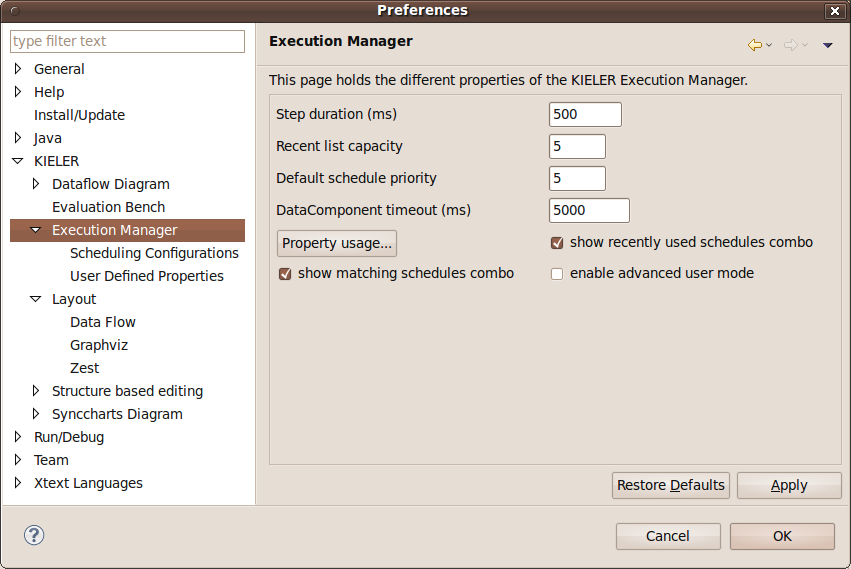
\includegraphics[scale=.45]{ConfigurationPage.png}
  \caption[The main preference page of the Execution Manager]%
  {The main preference page of the Execution Manager\protect}
  \label{fig:ConfigurationPage}
\end{figure}
On the main preference page of the Execution Manager shown in Figure \ref{fig:ConfigurationPage} the user can
set up most of the default properties. The user can also change the visibility of the ComboBoxes that display
the recently used and matching schedules. The last CheckBox is for enabling the advanced user mode.

In the normal user mode the ConfigDataComponent described in Section \ref{section:ConfigDataComponent} is
not visible to the user. It is also automatically added to any new file that is loaded into the Execution Manager.
While this behavior is fine for the average user an advanced user may want to have a little more control. An advantage
of having the component visible is that the user can reinitialize the current configuration with the values in
the default configuration by removing and adding the component in the list.


\subsubsection{User-Defined Properties Page}
\label{section:UserDefinedPropertiesPage}
\begin{figure}[User-Defined Properties Page]
  \centering
  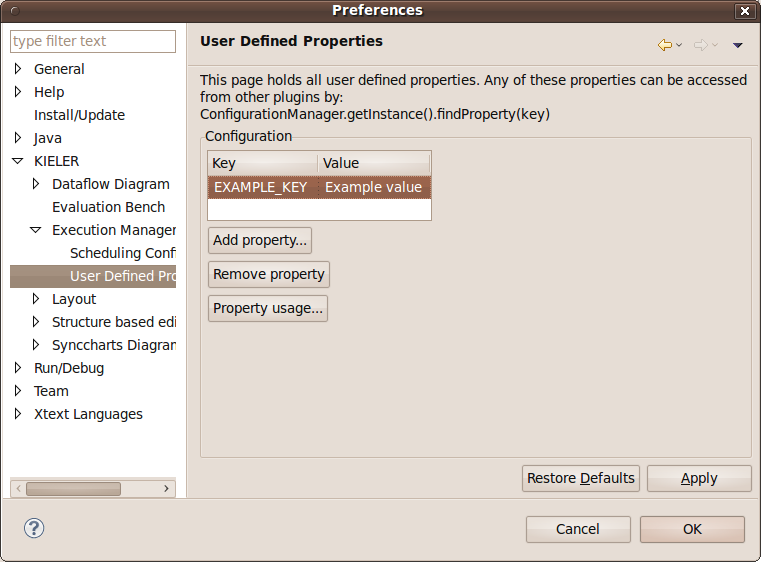
\includegraphics[scale=.5]{UserPropertiesPage.png}
  \caption[The page for defining custom properties]%
  {The page for defining custom properties\protect}
  \label{fig:UserDefinedPropertiesPage}
\end{figure}
Since there is a page to modify the internal properties of the Execution Manager there also exists a
preference page where the user can define, edit and remove his own properties (see Figure \ref{fig:UserDefinedPropertiesPage}). 
These properties can then be accessed by any DataComponent (or any other plug-in) through the \ac{KIEMConfig}'s \ac{API}.

Since not much can be said about the nature of the user defined properties there is no real format that
can be chosen for an individual property. Thus all properties are simply displayed in a table with a 
key and a value column. 

The user is only allowed to edit the value column of previously defined properties. This restriction is
necessary to keep the user from accidentally changing keys that are required by another users DataComponent.

However the user can remove a property that is no longer needed or define his own properties with a custom key.

\subsubsection{Property Usage Dialog}
Both of the previously described pages contain a button for accessing the Property Usage Dialog.
This dialog (see figure \ref{fig:PropertyUsageDialog}) is used for selecting which properties should always be taken
from the default configuration rather than the configuration component contained in every .execution file.
The dialog used for this is a ListSelectionDialog which just receives the list of
all keys as input and the list of PropertyKeys from the PropertyUsageManager as default selection.
After the user is finished with selecting attributes and hit the 'Ok' Button the dialog
passes the new list of selected items back to the PropertyUsageManager.
\begin{figure}[PropertyUsageDialog]
  \centering
  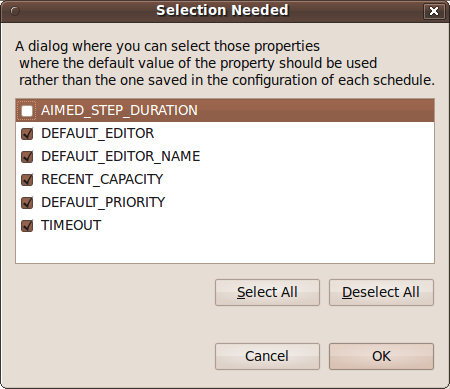
\includegraphics[scale=.5]{PropertyUsageDialog.png}
  \caption[Property Usage Dialog]%
  {The Property Usage Dialog\protect}
  \label{fig:PropertyUsageDialog}
\end{figure}

\subsection{Scheduling Page}
\label{section:SchedulingPage}
\index{Scheduling Page}
\begin{figure}[Scheduling Page]
  \centering
  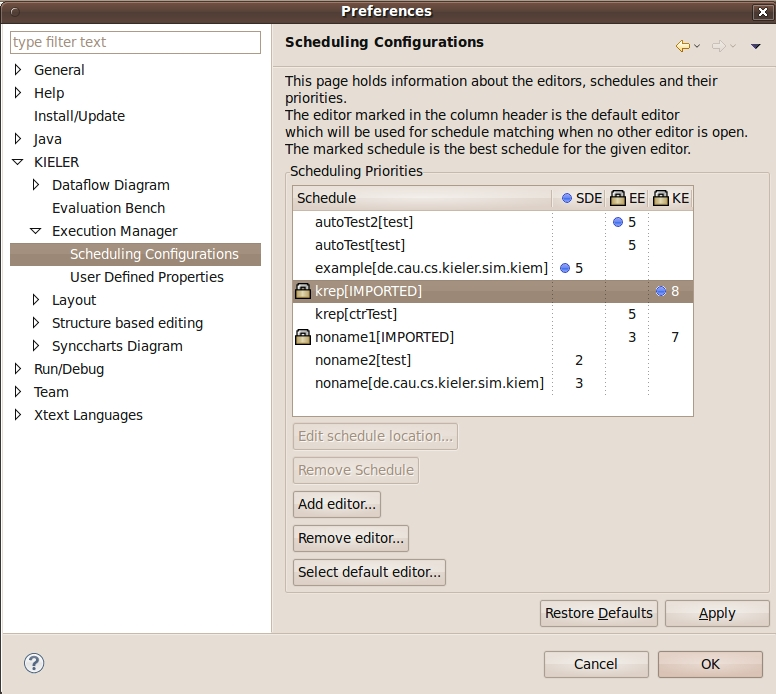
\includegraphics[scale=.45]{SchedulePage.jpg}
  \caption[The page for managing the schedules and editors]%
  {The page for managing the schedules and editors\protect}
  \label{fig:SchedulePage}
\end{figure}
This preference page (see Figure \ref{fig:SchedulePage} is used to manage the schedules and the editors that they belong to.
As mentioned in Section \ref{section:ConfConceptsDefaultConf} this page is basically a modified version 
of the LayoutPrioritiesPage by Miro Sp\"onemann (see Figure \ref{fig:MSPLayoutPreferencePage}).

The page is divided into two parts. The top part shows the table, the bottom part the buttons for manipulating
the table entries.

The table column headers show the abbreviated names of the editors (the tool tip of each header will show the full name). 
Each column represents the priorities that the different schedules have for this particular editor. When the editor is
active in the workbench view the list of matching schedules will be sorted in the order of these priorities. The user
can directly edit these properties in the table. For easier readability the best schedule for each editor is marked
with a dot and the table is sortable by clicking any of the column headers.

The editors and schedules that have a padlock next to their name are the ones imported through the default schedule 
extension point described in Section \ref{section:DefaultSchedule}. These editors and schedules are not supposed
to be edited or removed since they represent a factory default setting. The view realizes this by graying out the 
corresponding buttons when an imported schedule is selected.

All other schedules can be removed by simply clicking the appropriate button. The button for editing the location
of a schedule opens a dialog showing the currently active workspace and allows the user to select a new
execution file that should be associated with the selected schedule. This feature is necessary in case the user
moves a schedule through his file browser instead of the refactoring facilities on the workbench.

The editor marked with the dot is the default editor (see Section \ref{section:DefaultEditor}.

\subsubsection{Adding and Removing Editors, Selecting a Default Editor}
\begin{figure}[EditorSelectionDialog]
  \centering
  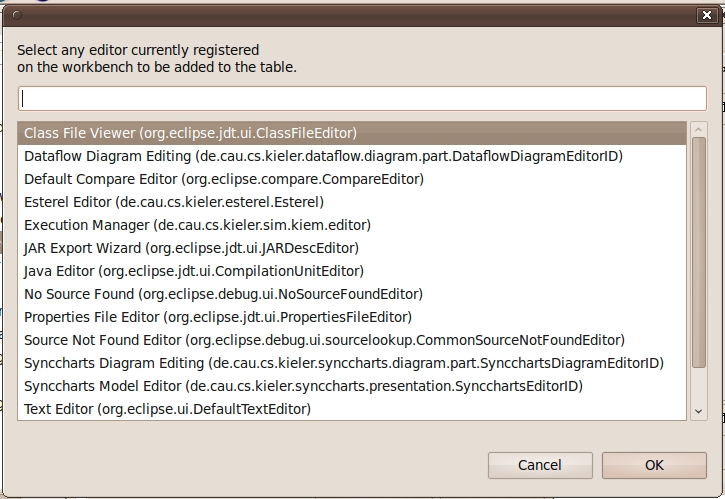
\includegraphics[scale=.5]{EditorSelectionDialog.jpg}
  \caption[Editor Selection Dialog]%
  {The Editor Selection Dialog\protect}
  \label{fig:EditorSelectionDialog}
\end{figure}

On the scheduling preference page there are routines for adding and removing
editors as well as selecting a default editor.
All of these actions use the same basic method for displaying an ElementListSelectionDialog \ref{fig:EditorSelectionDialog}
that takes a list of editor ids and returns the one selected by the user.
\begin{itemize}
 \item The editor adding dialog gets a list of all editors currently registered on the
 active workbench. The user can select a single editor which is then added to the table.
 \item The editor removal dialog gets a list of all editors currently available for 
 assignment of support properties. The editor selected by the user is removed from the table.
 It is also removed from all schedules. This is done to prevent the schedule objects from growing
 to unnecessarily large size over time when editors are getting added and removed.
 \item The default editor selection dialog gets the same list as the removal dialog. The selected
 editor is then set as default editor. 
\end{itemize}


\subsection{Schedule Selector}
\label{section:ScheduleSelector}
\index{Schedule Selector}
\begin{figure}[Schedule Selector]
  \centering
  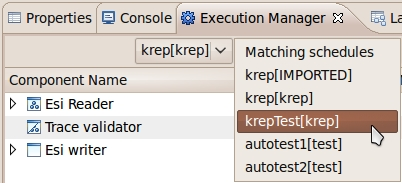
\includegraphics[scale=.5]{ScheduleSelector.jpg}
  \caption[The Schedule Selection ComboBoxes]%
  {The Schedule Selection ComboBoxes\protect}
  \label{fig:ScheduleSelector}
\end{figure}
The Schedule Selector is the only view element isn't shown on the preference pages. It is used
to construct and manage the two ComboBoxes for loading schedules that are known to
the \ac{KIEMConfig}. Each of the two ComboBoxes seen in Figure \ref{fig:ScheduleSelector} has its own task.
\begin{description}
 \item \textbf{The Matching Selector} : This ComboBox displays the schedules that can be used with
the currently active editor. The list is sorted by the priorities assigned through the preference page.
It displays a header showing its purpose in order to distinguish it from the other ComboBox.
 \item \textbf{The Recently Used Selector} : This ComboBox displays the list of recently used schedules.
The list is ordered in the same order that the schedules have been accessed through the Execution Manager.
The maximum size of the list can be configured through the preference page. The ComboBox displays the name
of the currently loaded execution file regardless of how it was loaded. This was done because up till now 
there actually was no way to tell which execution file was loaded in the Execution Manager.
\end{description}

